\section*{Assignment 08: Metrics and Learning}
\addcontentsline{toc}{section}{Assignment 08: Metrics and Learning}

\subsection*{Choosing metrics with intent}
I selected metrics using the decision tree from Lecture~5 \citep{Lecture05}: start with the core interaction, then layer retention, monetisation, and fairness signals. Each metric below includes the behaviour it captures and the follow up action.
\begin{itemize}
    \item \textbf{Matching rate.} Share of suggested matches that convert into accepted projects. If the rate falls, the team inspects the scoping wizard logs and interview transcripts to see whether prompts confuse users.
    \item \textbf{Repeat usage within thirty days.} Tracks whether students and organisations return quickly. A drop triggers outreach interviews and a review of community rituals.
    \item \textbf{Net promoter score.} Captures trust sentiment. Scores below plus twenty launch a qualitative survey and a moderation audit, reflecting \citet{Choudary2016}'s warning that trust is the oxygen of network effects.
    \item \textbf{Time to first value.} Measures minutes from signup to first meaningful action. If it exceeds thirty minutes we simplify the onboarding checklist or add live support.
    \item \textbf{Revenue per active match.} Keeps monetisation tied to delivered value. Sudden spikes prompt a fairness review to ensure a few large partners are not masking churn elsewhere.
    \item \textbf{Equity of participation.} Calculates the share of projects coming from resource light partners, using the fairness clause definitions from Assignment~07. A decline leads to additional subsidies or outreach.
    \item \textbf{Partner retention within sixty days.} Ensures NGOs stay engaged. If it slides, the partner success team runs structured exit interviews and updates the assurance programme.
\end{itemize}

\subsection*{Data infrastructure and rituals}
The data stack mirrors the minimal viable analytics architecture discussed in Lecture~5. Events flow through Segment or RudderStack into a warehouse such as BigQuery. Transformation happens in dbt with version controlled SQL so definitions stay transparent. Dashboards live in Metabase with row level permissions. Every chart includes a tooltip that links to the metric specification document.

Three cadences keep learning alive. Weekly reviews bring product, data, and support together to inspect dashboard slices and new cohort behaviour. Monthly cohort analyses segment users by acquisition channel and project type to spot retention differences. Quarterly learning reviews summarise experiments, capture lessons learned, and refresh hypotheses. These rituals replicate the "measure, learn, adapt" rhythm \citet{Choudary2016} advocates.

\subsection*{From metrics to action}
To illustrate the loop, imagine matching rate dropping from sixty two percent to forty eight percent over three weeks. Weekly review notes show that new users from a faculty campaign stall at the preference step and that time to first value exceeds forty five minutes. The team launches an onboarding A B test that adds a guided preference picker, reruns matching weights to favour recent activity, and schedules office hours for the affected cohort. Success criteria include matching rate returning above sixty percent, repeat usage improving by eight points, and equity of participation holding steady. Figure~\ref{fig:feedback-screen} shows the feedback interface that generates the qualitative data needed for these adjustments.

\begin{figure}[H]
  \centering
  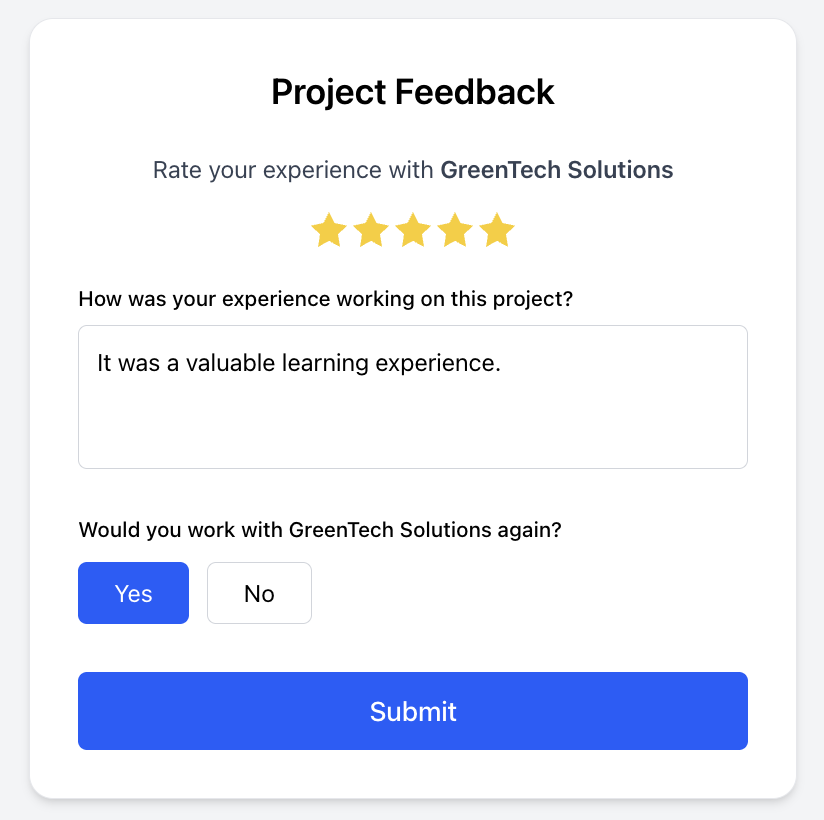
\includegraphics[width=0.8\linewidth]{figures/Student-Project-Feedback.png}
  \caption{Feedback screen mock up balancing qualitative notes and structured scores.}
  \label{fig:feedback-screen}
\end{figure}

Documentation practices close the loop. Metric definitions live in a public wiki, SQL is stored in Git, and quarterly snapshots archive the state of each KPI. That discipline makes the analytics reproducible and keeps future contributors accountable to the same definitions \citep{Choudary2016}.
